\documentclass[twoside]{book}

% Packages required by doxygen
\usepackage{fixltx2e}
\usepackage{calc}
\usepackage{doxygen}
\usepackage[export]{adjustbox} % also loads graphicx
\usepackage{graphicx}
\usepackage[utf8]{inputenc}
\usepackage{makeidx}
\usepackage{multicol}
\usepackage{multirow}
\PassOptionsToPackage{warn}{textcomp}
\usepackage{textcomp}
\usepackage[nointegrals]{wasysym}
\usepackage[table]{xcolor}

% Font selection
\usepackage[T1]{fontenc}
\usepackage[scaled=.90]{helvet}
\usepackage{courier}
\usepackage{amssymb}
\usepackage{sectsty}
\renewcommand{\familydefault}{\sfdefault}
\allsectionsfont{%
  \fontseries{bc}\selectfont%
  \color{darkgray}%
}
\renewcommand{\DoxyLabelFont}{%
  \fontseries{bc}\selectfont%
  \color{darkgray}%
}
\newcommand{\+}{\discretionary{\mbox{\scriptsize$\hookleftarrow$}}{}{}}

% Page & text layout
\usepackage{geometry}
\geometry{%
  a4paper,%
  top=2.5cm,%
  bottom=2.5cm,%
  left=2.5cm,%
  right=2.5cm%
}
\tolerance=750
\hfuzz=15pt
\hbadness=750
\setlength{\emergencystretch}{15pt}
\setlength{\parindent}{0cm}
\setlength{\parskip}{3ex plus 2ex minus 2ex}
\makeatletter
\renewcommand{\paragraph}{%
  \@startsection{paragraph}{4}{0ex}{-1.0ex}{1.0ex}{%
    \normalfont\normalsize\bfseries\SS@parafont%
  }%
}
\renewcommand{\subparagraph}{%
  \@startsection{subparagraph}{5}{0ex}{-1.0ex}{1.0ex}{%
    \normalfont\normalsize\bfseries\SS@subparafont%
  }%
}
\makeatother

% Headers & footers
\usepackage{fancyhdr}
\pagestyle{fancyplain}
\fancyhead[LE]{\fancyplain{}{\bfseries\thepage}}
\fancyhead[CE]{\fancyplain{}{}}
\fancyhead[RE]{\fancyplain{}{\bfseries\leftmark}}
\fancyhead[LO]{\fancyplain{}{\bfseries\rightmark}}
\fancyhead[CO]{\fancyplain{}{}}
\fancyhead[RO]{\fancyplain{}{\bfseries\thepage}}
\fancyfoot[LE]{\fancyplain{}{}}
\fancyfoot[CE]{\fancyplain{}{}}
\fancyfoot[RE]{\fancyplain{}{\bfseries\scriptsize Generated by Doxygen }}
\fancyfoot[LO]{\fancyplain{}{\bfseries\scriptsize Generated by Doxygen }}
\fancyfoot[CO]{\fancyplain{}{}}
\fancyfoot[RO]{\fancyplain{}{}}
\renewcommand{\footrulewidth}{0.4pt}
\renewcommand{\chaptermark}[1]{%
  \markboth{#1}{}%
}
\renewcommand{\sectionmark}[1]{%
  \markright{\thesection\ #1}%
}

% Indices & bibliography
\usepackage{natbib}
\usepackage[titles]{tocloft}
\setcounter{tocdepth}{3}
\setcounter{secnumdepth}{5}
\makeindex

% Hyperlinks (required, but should be loaded last)
\usepackage{ifpdf}
\ifpdf
  \usepackage[pdftex,pagebackref=true]{hyperref}
\else
  \usepackage[ps2pdf,pagebackref=true]{hyperref}
\fi
\hypersetup{%
  colorlinks=true,%
  linkcolor=blue,%
  citecolor=blue,%
  unicode%
}

% Custom commands
\newcommand{\clearemptydoublepage}{%
  \newpage{\pagestyle{empty}\cleardoublepage}%
}

\usepackage{caption}
\captionsetup{labelsep=space,justification=centering,font={bf},singlelinecheck=off,skip=4pt,position=top}

%===== C O N T E N T S =====

\begin{document}

% Titlepage & ToC
\hypersetup{pageanchor=false,
             bookmarksnumbered=true,
             pdfencoding=unicode
            }
\pagenumbering{roman}
\begin{titlepage}
\vspace*{7cm}
\begin{center}%
{\Large 山火-\/ヤギの咆哮-\/ }\\
\vspace*{1cm}
{\large Generated by Doxygen 1.8.11}\\
\end{center}
\end{titlepage}
\clearemptydoublepage
\tableofcontents
\clearemptydoublepage
\pagenumbering{arabic}
\hypersetup{pageanchor=true}

%--- Begin generated contents ---
\chapter{Hierarchical Index}
\section{Class Hierarchy}
This inheritance list is sorted roughly, but not completely, alphabetically\+:\begin{DoxyCompactList}
\item \contentsline{section}{Draw\+System}{\pageref{class_draw_system}}{}
\item enable\+\_\+shared\+\_\+from\+\_\+this\begin{DoxyCompactList}
\item \contentsline{section}{Sprite}{\pageref{class_sprite}}{}
\end{DoxyCompactList}
\item \contentsline{section}{Graphics\+Manager}{\pageref{class_graphics_manager}}{}
\item I\+File\+Load\+Listener\begin{DoxyCompactList}
\item \contentsline{section}{Font\+Sprite\+Texture\+Loader}{\pageref{class_font_sprite_texture_loader}}{}
\end{DoxyCompactList}
\item \contentsline{section}{Input\+Manager}{\pageref{class_input_manager}}{}
\item \contentsline{section}{Lua\+Helper}{\pageref{class_lua_helper}}{}
\item \contentsline{section}{My\+Framework}{\pageref{class_my_framework}}{}
\item \contentsline{section}{Properties}{\pageref{class_properties}}{}
\item \contentsline{section}{Simple\+Helpers}{\pageref{class_simple_helpers}}{}
\item \contentsline{section}{Sound\+Manager}{\pageref{class_sound_manager}}{}
\end{DoxyCompactList}

\chapter{Class Index}
\section{Class List}
Here are the classes, structs, unions and interfaces with brief descriptions\+:\begin{DoxyCompactList}
\item\contentsline{section}{\hyperlink{class_draw_system}{Draw\+System} \\*描画システムを提供する }{\pageref{class_draw_system}}{}
\item\contentsline{section}{\hyperlink{class_font_sprite_texture_loader}{Font\+Sprite\+Texture\+Loader} }{\pageref{class_font_sprite_texture_loader}}{}
\item\contentsline{section}{\hyperlink{class_graphics_manager}{Graphics\+Manager} \\*画像の読み込み、破棄をコントロールする。インスタンスは一つのみ持つ。 }{\pageref{class_graphics_manager}}{}
\item\contentsline{section}{\hyperlink{class_input_manager}{Input\+Manager} \\*キーボードの入力情報を管理する }{\pageref{class_input_manager}}{}
\item\contentsline{section}{\hyperlink{class_lua_helper}{Lua\+Helper} \\*Luaを便利に利用するための機能を提供する }{\pageref{class_lua_helper}}{}
\item\contentsline{section}{\hyperlink{class_my_framework}{My\+Framework} \\*ゲームフレームワーク }{\pageref{class_my_framework}}{}
\item\contentsline{section}{\hyperlink{class_properties}{Properties} \\*ゲームのプロパティ }{\pageref{class_properties}}{}
\item\contentsline{section}{\hyperlink{class_simple_helpers}{Simple\+Helpers} \\*細々としたヘルパー群 }{\pageref{class_simple_helpers}}{}
\item\contentsline{section}{\hyperlink{class_sound_manager}{Sound\+Manager} \\*B\+G\+M・効果音の読み込み、破棄をコントロールする。インスタンスは一つのみ持つ。 }{\pageref{class_sound_manager}}{}
\item\contentsline{section}{\hyperlink{class_sprite}{Sprite} \\*スプライト機能を提供する }{\pageref{class_sprite}}{}
\end{DoxyCompactList}

\chapter{Class Documentation}
\hypertarget{class_draw_system}{}\section{Draw\+System Class Reference}
\label{class_draw_system}\index{Draw\+System@{Draw\+System}}


描画システムを提供する  




{\ttfamily \#include $<$Sprite\+Node.\+hpp$>$}

\subsection*{Public Member Functions}
\begin{DoxyCompactItemize}
\item 
bool {\bfseries On\+Power\+Init} ()\hypertarget{class_draw_system_a4fcc569cfd3066844254eb1c06e72f20}{}\label{class_draw_system_a4fcc569cfd3066844254eb1c06e72f20}

\item 
void {\bfseries Dispose} ()\hypertarget{class_draw_system_a3ac28af10a2f61a4fa54e4230f3afb8e}{}\label{class_draw_system_a3ac28af10a2f61a4fa54e4230f3afb8e}

\item 
boost\+::shared\+\_\+ptr$<$ \hyperlink{class_sprite}{Sprite} $>$ {\bfseries Get\+Sprite} ()\hypertarget{class_draw_system_a81593792372d8793a9204547e3eb5582}{}\label{class_draw_system_a81593792372d8793a9204547e3eb5582}

\item 
void {\bfseries Add\+Sprite} (boost\+::shared\+\_\+ptr$<$ \hyperlink{class_sprite}{Sprite} $>$ spr)\hypertarget{class_draw_system_aec142a500ca3cfa0f58c57ec4f40cf3a}{}\label{class_draw_system_aec142a500ca3cfa0f58c57ec4f40cf3a}

\item 
void {\bfseries Remove\+Sprite} (boost\+::shared\+\_\+ptr$<$ \hyperlink{class_sprite}{Sprite} $>$ spr)\hypertarget{class_draw_system_a558dcef6044d9d747056af003d889870}{}\label{class_draw_system_a558dcef6044d9d747056af003d889870}

\item 
void {\bfseries Clear\+Sprite} ()\hypertarget{class_draw_system_a9332ac89fa32d17bf7dfd09bbfa573ae}{}\label{class_draw_system_a9332ac89fa32d17bf7dfd09bbfa573ae}

\item 
void {\bfseries Draw} ()\hypertarget{class_draw_system_a39cef1b6e860faeddd1b88748fec0e0f}{}\label{class_draw_system_a39cef1b6e860faeddd1b88748fec0e0f}

\end{DoxyCompactItemize}
\subsection*{Static Public Member Functions}
\begin{DoxyCompactItemize}
\item 
static \hyperlink{class_draw_system}{Draw\+System} $\ast$ {\bfseries Get\+Inst} ()\hypertarget{class_draw_system_a2fc7f9c286b296a186df6dc1824291e6}{}\label{class_draw_system_a2fc7f9c286b296a186df6dc1824291e6}

\item 
static void {\bfseries Regist\+Lua} ()\hypertarget{class_draw_system_aea7beebfb1c694ad8ae23aa5128445b0}{}\label{class_draw_system_aea7beebfb1c694ad8ae23aa5128445b0}

\end{DoxyCompactItemize}


\subsection{Detailed Description}
描画システムを提供する 

The documentation for this class was generated from the following files\+:\begin{DoxyCompactItemize}
\item 
山火-\/ヤギの咆哮-\//Sprite\+Node.\+hpp\item 
山火-\/ヤギの咆哮-\//Sprite\+Node.\+cpp\end{DoxyCompactItemize}

\hypertarget{class_font_sprite_texture_loader}{}\section{Font\+Sprite\+Texture\+Loader Class Reference}
\label{class_font_sprite_texture_loader}\index{Font\+Sprite\+Texture\+Loader@{Font\+Sprite\+Texture\+Loader}}
Inheritance diagram for Font\+Sprite\+Texture\+Loader\+:\begin{figure}[H]
\begin{center}
\leavevmode
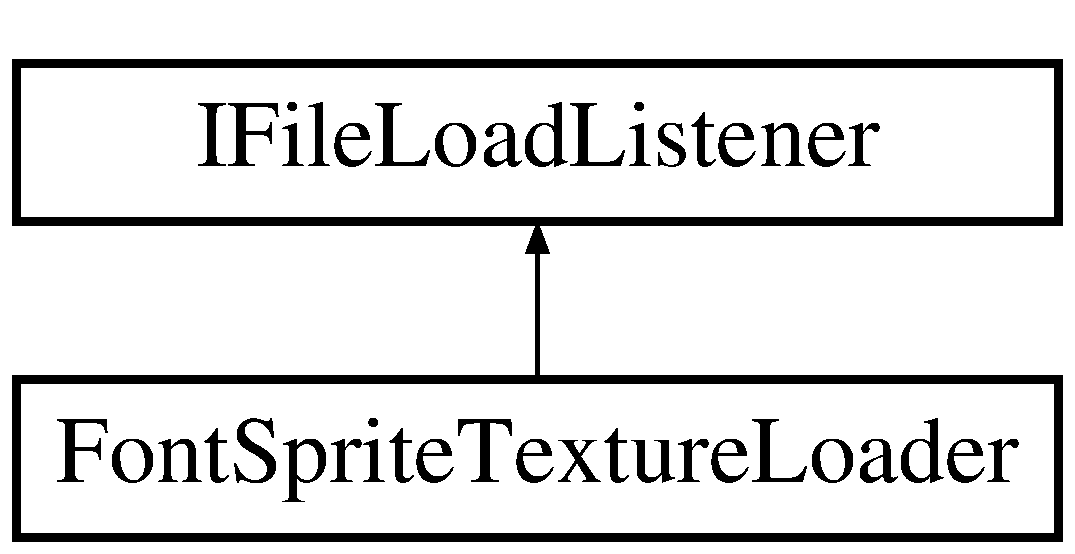
\includegraphics[height=2.000000cm]{class_font_sprite_texture_loader}
\end{center}
\end{figure}


The documentation for this class was generated from the following file\+:\begin{DoxyCompactItemize}
\item 
山火-\/ヤギの咆哮-\//Graphics\+Manager.\+cpp\end{DoxyCompactItemize}

\hypertarget{class_graphics_manager}{}\section{Graphics\+Manager Class Reference}
\label{class_graphics_manager}\index{Graphics\+Manager@{Graphics\+Manager}}


画像の読み込み、破棄をコントロールする。インスタンスは一つのみ持つ。  




{\ttfamily \#include $<$Graphics\+Manager.\+hpp$>$}

\subsection*{Public Member Functions}
\begin{DoxyCompactItemize}
\item 
bool \hyperlink{class_graphics_manager_a3855839d0ac22373eb85a821f88d7f77}{On\+Power\+Init} (Graphics\+::\+I\+Manager $\ast$mgr)\hypertarget{class_graphics_manager_a3855839d0ac22373eb85a821f88d7f77}{}\label{class_graphics_manager_a3855839d0ac22373eb85a821f88d7f77}

\begin{DoxyCompactList}\small\item\em ゲーム起動時の初期化を行う \end{DoxyCompactList}\item 
void \hyperlink{class_graphics_manager_aaffde352f9d9edcb7bc00c756b5ff7ec}{Dispose} ()\hypertarget{class_graphics_manager_aaffde352f9d9edcb7bc00c756b5ff7ec}{}\label{class_graphics_manager_aaffde352f9d9edcb7bc00c756b5ff7ec}

\begin{DoxyCompactList}\small\item\em 読み込んだリソースを破棄する \end{DoxyCompactList}\item 
void \hyperlink{class_graphics_manager_a5aaa3946913d78085220f1c112da82ca}{Load\+Texture} (const std\+::string path, const std\+::string name)
\item 
void \hyperlink{class_graphics_manager_a6d53401e0d3ef8f187ee7db70270056d}{Load\+Texture2} (const std\+::string path, const std\+::string name)
\item 
void \hyperlink{class_graphics_manager_a0dff6d46fc42021eba1d81d72c6946ed}{Load\+Font} (const std\+::string path, const std\+::string font\+Name, const std\+::string regist\+Name)
\item 
Texture $\ast$ \hyperlink{class_graphics_manager_a5fe2ed3a63f3cb65031b3d37c4dd3f0a}{Get\+Texture} (const std\+::string name)\hypertarget{class_graphics_manager_a5fe2ed3a63f3cb65031b3d37c4dd3f0a}{}\label{class_graphics_manager_a5fe2ed3a63f3cb65031b3d37c4dd3f0a}

\begin{DoxyCompactList}\small\item\em 指定した名前の画像を取得する \end{DoxyCompactList}\item 
Point2\+DI \hyperlink{class_graphics_manager_a42562ffd6abcab5004c37c7f0618d423}{Get\+Texture\+Size} (const std\+::string name)\hypertarget{class_graphics_manager_a42562ffd6abcab5004c37c7f0618d423}{}\label{class_graphics_manager_a42562ffd6abcab5004c37c7f0618d423}

\begin{DoxyCompactList}\small\item\em 指定した名前の画像の大きさを取得する \end{DoxyCompactList}\item 
Graphics\+::\+Simple\+::\+I\+Text\+Renderer $\ast$ \hyperlink{class_graphics_manager_a065f94529b70f799553df3072ceac127}{Get\+Text\+Renderer} (std\+::string font, int size)\hypertarget{class_graphics_manager_a065f94529b70f799553df3072ceac127}{}\label{class_graphics_manager_a065f94529b70f799553df3072ceac127}

\begin{DoxyCompactList}\small\item\em フォント、文字サイズを指定してテキストレンダラーを取得する \end{DoxyCompactList}\item 
Text\+Data $\ast$ \hyperlink{class_graphics_manager_a68d7a473286bc1fa1241c3218e8d34ba}{Get\+Text\+Data} (std\+::string font)\hypertarget{class_graphics_manager_a68d7a473286bc1fa1241c3218e8d34ba}{}\label{class_graphics_manager_a68d7a473286bc1fa1241c3218e8d34ba}

\begin{DoxyCompactList}\small\item\em テキスト描画用データを取得する \end{DoxyCompactList}\item 
void \hyperlink{class_graphics_manager_a819093e6f8ee7413de0ef25be2877f60}{Remove\+Texture} (const std\+::string name)\hypertarget{class_graphics_manager_a819093e6f8ee7413de0ef25be2877f60}{}\label{class_graphics_manager_a819093e6f8ee7413de0ef25be2877f60}

\begin{DoxyCompactList}\small\item\em 指定した名前の画像を破棄する \end{DoxyCompactList}\item 
void \hyperlink{class_graphics_manager_a0bbe7909f7987bb838adbc8c034ca175}{Clear\+Texture} ()\hypertarget{class_graphics_manager_a0bbe7909f7987bb838adbc8c034ca175}{}\label{class_graphics_manager_a0bbe7909f7987bb838adbc8c034ca175}

\begin{DoxyCompactList}\small\item\em 読み込んだ画像を全て破棄する \end{DoxyCompactList}\item 
Graphics\+::\+I\+Manager $\ast$ {\bfseries Get\+Selene\+Gr\+Mgr} ()\hypertarget{class_graphics_manager_a2b025fce8ae30d8348ee5808b003c059}{}\label{class_graphics_manager_a2b025fce8ae30d8348ee5808b003c059}

\item 
Graphics\+::\+Simple\+::\+I\+Sprite\+Renderer $\ast$ {\bfseries Get\+Sprite} ()\hypertarget{class_graphics_manager_a72ab812dcc17d07a03a094e943ae3d2a}{}\label{class_graphics_manager_a72ab812dcc17d07a03a094e943ae3d2a}

\end{DoxyCompactItemize}
\subsection*{Static Public Member Functions}
\begin{DoxyCompactItemize}
\item 
static \hyperlink{class_graphics_manager}{Graphics\+Manager} $\ast$ \hyperlink{class_graphics_manager_a09b2f99634be4c527cd1f0071e9760df}{Get\+Inst} ()\hypertarget{class_graphics_manager_a09b2f99634be4c527cd1f0071e9760df}{}\label{class_graphics_manager_a09b2f99634be4c527cd1f0071e9760df}

\begin{DoxyCompactList}\small\item\em インスタンスを取得する \end{DoxyCompactList}\item 
static void \hyperlink{class_graphics_manager_ac4260b1d9469a88564ad948cdaca9d21}{Regist\+Lua} ()\hypertarget{class_graphics_manager_ac4260b1d9469a88564ad948cdaca9d21}{}\label{class_graphics_manager_ac4260b1d9469a88564ad948cdaca9d21}

\begin{DoxyCompactList}\small\item\em Luaで使用する機能を登録する \end{DoxyCompactList}\end{DoxyCompactItemize}


\subsection{Detailed Description}
画像の読み込み、破棄をコントロールする。インスタンスは一つのみ持つ。 

\subsection{Member Function Documentation}
\index{Graphics\+Manager@{Graphics\+Manager}!Load\+Font@{Load\+Font}}
\index{Load\+Font@{Load\+Font}!Graphics\+Manager@{Graphics\+Manager}}
\subsubsection[{\texorpdfstring{Load\+Font(const std\+::string path, const std\+::string font\+Name, const std\+::string regist\+Name)}{LoadFont(const std::string path, const std::string fontName, const std::string registName)}}]{\setlength{\rightskip}{0pt plus 5cm}void Graphics\+Manager\+::\+Load\+Font (
\begin{DoxyParamCaption}
\item[{const std\+::string}]{path, }
\item[{const std\+::string}]{font\+Name, }
\item[{const std\+::string}]{regist\+Name}
\end{DoxyParamCaption}
)}\hypertarget{class_graphics_manager_a0dff6d46fc42021eba1d81d72c6946ed}{}\label{class_graphics_manager_a0dff6d46fc42021eba1d81d72c6946ed}
フォントを読み込む 
\begin{DoxyParams}{Parameters}
{\em path} & 読み込むフォントデータのファイルパス \\
\hline
{\em font\+Name} & 読み込んだフォントの名前 \\
\hline
{\em register\+Name} & 読み込んだフォントを使用する際のエイリアス \\
\hline
\end{DoxyParams}
\index{Graphics\+Manager@{Graphics\+Manager}!Load\+Texture@{Load\+Texture}}
\index{Load\+Texture@{Load\+Texture}!Graphics\+Manager@{Graphics\+Manager}}
\subsubsection[{\texorpdfstring{Load\+Texture(const std\+::string path, const std\+::string name)}{LoadTexture(const std::string path, const std::string name)}}]{\setlength{\rightskip}{0pt plus 5cm}void Graphics\+Manager\+::\+Load\+Texture (
\begin{DoxyParamCaption}
\item[{const std\+::string}]{path, }
\item[{const std\+::string}]{name}
\end{DoxyParamCaption}
)}\hypertarget{class_graphics_manager_a5aaa3946913d78085220f1c112da82ca}{}\label{class_graphics_manager_a5aaa3946913d78085220f1c112da82ca}
画像を読み込む(上書き有り) 
\begin{DoxyParams}{Parameters}
{\em path} & 読み込む画像のファイルパス \\
\hline
{\em name} & 読み込んだ画像を使用する際のエイリアス \\
\hline
\end{DoxyParams}
\index{Graphics\+Manager@{Graphics\+Manager}!Load\+Texture2@{Load\+Texture2}}
\index{Load\+Texture2@{Load\+Texture2}!Graphics\+Manager@{Graphics\+Manager}}
\subsubsection[{\texorpdfstring{Load\+Texture2(const std\+::string path, const std\+::string name)}{LoadTexture2(const std::string path, const std::string name)}}]{\setlength{\rightskip}{0pt plus 5cm}void Graphics\+Manager\+::\+Load\+Texture2 (
\begin{DoxyParamCaption}
\item[{const std\+::string}]{path, }
\item[{const std\+::string}]{name}
\end{DoxyParamCaption}
)}\hypertarget{class_graphics_manager_a6d53401e0d3ef8f187ee7db70270056d}{}\label{class_graphics_manager_a6d53401e0d3ef8f187ee7db70270056d}
画像を読み込む(上書き無し) 
\begin{DoxyParams}{Parameters}
{\em path} & 読み込む画像のファイルパス \\
\hline
{\em name} & 読み込んだ画像を使用する際のエイリアス \\
\hline
\end{DoxyParams}


The documentation for this class was generated from the following files\+:\begin{DoxyCompactItemize}
\item 
山火-\/ヤギの咆哮-\//Graphics\+Manager.\+hpp\item 
山火-\/ヤギの咆哮-\//Graphics\+Manager.\+cpp\end{DoxyCompactItemize}

\hypertarget{class_input_manager}{}\section{Input\+Manager Class Reference}
\label{class_input_manager}\index{Input\+Manager@{Input\+Manager}}


キーボードの入力情報を管理する  




{\ttfamily \#include $<$Input\+Manager.\+hpp$>$}

\subsection*{Public Member Functions}
\begin{DoxyCompactItemize}
\item 
bool \hyperlink{class_input_manager_a9b808236f2b417d11aa255c03c7e21d7}{On\+Power\+Init} (Engine\+::\+Input\+::\+I\+Manager $\ast$mgr)\hypertarget{class_input_manager_a9b808236f2b417d11aa255c03c7e21d7}{}\label{class_input_manager_a9b808236f2b417d11aa255c03c7e21d7}

\begin{DoxyCompactList}\small\item\em ゲーム起動時の初期化を行う \end{DoxyCompactList}\item 
void \hyperlink{class_input_manager_aa5480931dba2720e7d80dd00a53adae0}{Update} ()\hypertarget{class_input_manager_aa5480931dba2720e7d80dd00a53adae0}{}\label{class_input_manager_aa5480931dba2720e7d80dd00a53adae0}

\begin{DoxyCompactList}\small\item\em キーボードの入力状況を更新する \end{DoxyCompactList}\item 
bool \hyperlink{class_input_manager_aefb7ea8dab0e99d26257b86e7ef98324}{Is\+Key\+Free} (Engine\+::\+Input\+::e\+Key\+Code key)\hypertarget{class_input_manager_aefb7ea8dab0e99d26257b86e7ef98324}{}\label{class_input_manager_aefb7ea8dab0e99d26257b86e7ef98324}

\begin{DoxyCompactList}\small\item\em キーが押されていなかったらtrue \end{DoxyCompactList}\item 
bool \hyperlink{class_input_manager_a25b4a91cf685997cf63d19262d2020ab}{Is\+Key\+Hold} (Engine\+::\+Input\+::e\+Key\+Code key)\hypertarget{class_input_manager_a25b4a91cf685997cf63d19262d2020ab}{}\label{class_input_manager_a25b4a91cf685997cf63d19262d2020ab}

\begin{DoxyCompactList}\small\item\em キーが押されていたらtrue \end{DoxyCompactList}\item 
bool \hyperlink{class_input_manager_a35a091d4deba839adbc4119796e7942c}{Is\+Key\+Pull} (Engine\+::\+Input\+::e\+Key\+Code key)\hypertarget{class_input_manager_a35a091d4deba839adbc4119796e7942c}{}\label{class_input_manager_a35a091d4deba839adbc4119796e7942c}

\begin{DoxyCompactList}\small\item\em キーが離された瞬間ならtrue \end{DoxyCompactList}\item 
bool \hyperlink{class_input_manager_a591e6e4c0644d0875b6a3fe4240a9fa2}{Is\+Key\+Push} (Engine\+::\+Input\+::e\+Key\+Code key)\hypertarget{class_input_manager_a591e6e4c0644d0875b6a3fe4240a9fa2}{}\label{class_input_manager_a591e6e4c0644d0875b6a3fe4240a9fa2}

\begin{DoxyCompactList}\small\item\em キーが押された瞬間ならtrue \end{DoxyCompactList}\item 
int \hyperlink{class_input_manager_a00f7496fc57f461bf8c0782a12771bc9}{Get\+Key\+Hold\+Cnt} (Engine\+::\+Input\+::e\+Key\+Code key)\hypertarget{class_input_manager_a00f7496fc57f461bf8c0782a12771bc9}{}\label{class_input_manager_a00f7496fc57f461bf8c0782a12771bc9}

\begin{DoxyCompactList}\small\item\em キーが押下されている継続フレームを取得する \end{DoxyCompactList}\item 
int \hyperlink{class_input_manager_a1d228312a8d269347a0a0346e8897ea9}{Get\+Key\+Free\+Cnt} (Engine\+::\+Input\+::e\+Key\+Code key)\hypertarget{class_input_manager_a1d228312a8d269347a0a0346e8897ea9}{}\label{class_input_manager_a1d228312a8d269347a0a0346e8897ea9}

\begin{DoxyCompactList}\small\item\em キーが離されている継続フレームを取得する \end{DoxyCompactList}\item 
bool \hyperlink{class_input_manager_addbd2d5a46ff66ec6dd759961bcca408}{Is\+Mouse\+Free} (e\+Mouse\+Button btn)\hypertarget{class_input_manager_addbd2d5a46ff66ec6dd759961bcca408}{}\label{class_input_manager_addbd2d5a46ff66ec6dd759961bcca408}

\begin{DoxyCompactList}\small\item\em マウスのボタンが押されていなかったらtrue \end{DoxyCompactList}\item 
bool \hyperlink{class_input_manager_afa182f53a9fb2461ebb25d0bf16addef}{Is\+Mouse\+Hold} (e\+Mouse\+Button btn)\hypertarget{class_input_manager_afa182f53a9fb2461ebb25d0bf16addef}{}\label{class_input_manager_afa182f53a9fb2461ebb25d0bf16addef}

\begin{DoxyCompactList}\small\item\em マウスのボタンが押されていたらtrue \end{DoxyCompactList}\item 
bool \hyperlink{class_input_manager_a4c3e08df40d0538f850f4d476643aeb7}{Is\+Mouse\+Pull} (e\+Mouse\+Button btn)\hypertarget{class_input_manager_a4c3e08df40d0538f850f4d476643aeb7}{}\label{class_input_manager_a4c3e08df40d0538f850f4d476643aeb7}

\begin{DoxyCompactList}\small\item\em マウスのボタンが離された瞬間ならtrue \end{DoxyCompactList}\item 
bool \hyperlink{class_input_manager_aac50cc157411461d9419925b777dfc90}{Is\+Mouse\+Click} (e\+Mouse\+Button btn)\hypertarget{class_input_manager_aac50cc157411461d9419925b777dfc90}{}\label{class_input_manager_aac50cc157411461d9419925b777dfc90}

\begin{DoxyCompactList}\small\item\em マウスのボタンがクリックされた瞬間ならtrue \end{DoxyCompactList}\item 
int \hyperlink{class_input_manager_a80cfed4ebb420ae2c9ea741b775a4673}{Get\+Mouse\+Hold\+Cnt} (e\+Mouse\+Button key)\hypertarget{class_input_manager_a80cfed4ebb420ae2c9ea741b775a4673}{}\label{class_input_manager_a80cfed4ebb420ae2c9ea741b775a4673}

\begin{DoxyCompactList}\small\item\em マウスのボタンが押下されている継続フレームを取得する \end{DoxyCompactList}\item 
int \hyperlink{class_input_manager_a5be0ced7a28a44e225ac7de50548bf93}{Get\+Mouse\+Free\+Cnt} (e\+Mouse\+Button key)\hypertarget{class_input_manager_a5be0ced7a28a44e225ac7de50548bf93}{}\label{class_input_manager_a5be0ced7a28a44e225ac7de50548bf93}

\begin{DoxyCompactList}\small\item\em マウスのボタンが離されている継続フレームを取得する \end{DoxyCompactList}\item 
Point2\+DI \hyperlink{class_input_manager_a0866591eebc6a5838433be4782cdac3d}{Get\+Mouse\+Pos} ()\hypertarget{class_input_manager_a0866591eebc6a5838433be4782cdac3d}{}\label{class_input_manager_a0866591eebc6a5838433be4782cdac3d}

\begin{DoxyCompactList}\small\item\em マウスカーソルの座標を取得する \end{DoxyCompactList}\item 
void {\bfseries Init\+On\+Power} ()\hypertarget{class_input_manager_ae50dda5e0e8f33f7a40665551eb6637f}{}\label{class_input_manager_ae50dda5e0e8f33f7a40665551eb6637f}

\end{DoxyCompactItemize}
\subsection*{Static Public Member Functions}
\begin{DoxyCompactItemize}
\item 
static \hyperlink{class_input_manager}{Input\+Manager} $\ast$ \hyperlink{class_input_manager_ae7f3e9db7e5a4d157930a717512f5c2e}{Get\+Inst} ()\hypertarget{class_input_manager_ae7f3e9db7e5a4d157930a717512f5c2e}{}\label{class_input_manager_ae7f3e9db7e5a4d157930a717512f5c2e}

\begin{DoxyCompactList}\small\item\em インスタンスを取得する \end{DoxyCompactList}\item 
static void \hyperlink{class_input_manager_a92b6a2082bdb95b5daf23b24aedfb0f6}{Regist\+Lua} ()\hypertarget{class_input_manager_a92b6a2082bdb95b5daf23b24aedfb0f6}{}\label{class_input_manager_a92b6a2082bdb95b5daf23b24aedfb0f6}

\begin{DoxyCompactList}\small\item\em Luaで使用する機能を登録する \end{DoxyCompactList}\end{DoxyCompactItemize}


\subsection{Detailed Description}
キーボードの入力情報を管理する 

The documentation for this class was generated from the following files\+:\begin{DoxyCompactItemize}
\item 
山火-\/ヤギの咆哮-\//Input\+Manager.\+hpp\item 
山火-\/ヤギの咆哮-\//Input\+Manager.\+cpp\end{DoxyCompactItemize}

\hypertarget{class_lua_helper}{}\section{Lua\+Helper Class Reference}
\label{class_lua_helper}\index{Lua\+Helper@{Lua\+Helper}}


Luaを便利に利用するための機能を提供する  




{\ttfamily \#include $<$Lua\+Helper.\+hpp$>$}

\subsection*{Public Member Functions}
\begin{DoxyCompactItemize}
\item 
lua\+\_\+\+State $\ast$ {\bfseries Get\+Lua} ()\hypertarget{class_lua_helper_a3738931605b20ba3a93884f29f7dbb04}{}\label{class_lua_helper_a3738931605b20ba3a93884f29f7dbb04}

\item 
bool \hyperlink{class_lua_helper_aca3c0411f11bec8d43ffade1837ba7aa}{Initialize} ()\hypertarget{class_lua_helper_aca3c0411f11bec8d43ffade1837ba7aa}{}\label{class_lua_helper_aca3c0411f11bec8d43ffade1837ba7aa}

\begin{DoxyCompactList}\small\item\em Luaを使用するための初期化を行う \end{DoxyCompactList}\item 
void \hyperlink{class_lua_helper_ad4d67528e295aff02653287258f2f1c3}{Close} ()\hypertarget{class_lua_helper_ad4d67528e295aff02653287258f2f1c3}{}\label{class_lua_helper_ad4d67528e295aff02653287258f2f1c3}

\begin{DoxyCompactList}\small\item\em 指定した\+Luaスクリプトを実行する \end{DoxyCompactList}\item 
bool \hyperlink{class_lua_helper_a153924ff92fba4630eeae6f75d197c9d}{Reload\+Lua\+Files} (\hyperlink{class_my_framework}{My\+Framework} $\ast$appli, const std\+::string reload\+Type)\hypertarget{class_lua_helper_a153924ff92fba4630eeae6f75d197c9d}{}\label{class_lua_helper_a153924ff92fba4630eeae6f75d197c9d}

\begin{DoxyCompactList}\small\item\em Luaスクリプトを読み込み直す \end{DoxyCompactList}\item 
bool \hyperlink{class_lua_helper_ab9bb186436aa630ccb055bce2ca85878}{Do\+File} (const std\+::string path)\hypertarget{class_lua_helper_ab9bb186436aa630ccb055bce2ca85878}{}\label{class_lua_helper_ab9bb186436aa630ccb055bce2ca85878}

\begin{DoxyCompactList}\small\item\em 指定した\+Luaスクリプトを実行する \end{DoxyCompactList}\item 
int \hyperlink{class_lua_helper_adfce384395bce376e1ebb57a849ced5e}{Error\+Callback} ()\hypertarget{class_lua_helper_adfce384395bce376e1ebb57a849ced5e}{}\label{class_lua_helper_adfce384395bce376e1ebb57a849ced5e}

\begin{DoxyCompactList}\small\item\em Luaスクリプトの実行中にエラーが発生した場合に呼び出される \end{DoxyCompactList}\item 
std\+::string \hyperlink{class_lua_helper_a78f86c10afc8de57ba10317599b1a4a6}{Get\+Err} ()\hypertarget{class_lua_helper_a78f86c10afc8de57ba10317599b1a4a6}{}\label{class_lua_helper_a78f86c10afc8de57ba10317599b1a4a6}

\begin{DoxyCompactList}\small\item\em 内部で保持しているエラーメッセージを取得する \end{DoxyCompactList}\item 
bool \hyperlink{class_lua_helper_a18972f326b9a1306513a58fad8dc9384}{Show\+Error\+Reload\+Dialog} (\hyperlink{class_my_framework}{My\+Framework} $\ast$appli, luabind\+::error e)
\end{DoxyCompactItemize}
\subsection*{Static Public Member Functions}
\begin{DoxyCompactItemize}
\item 
static \hyperlink{class_lua_helper}{Lua\+Helper} $\ast$ \hyperlink{class_lua_helper_add03b0c9e9c0f79d00c77fe4b2893fe8}{Get\+Inst} ()\hypertarget{class_lua_helper_add03b0c9e9c0f79d00c77fe4b2893fe8}{}\label{class_lua_helper_add03b0c9e9c0f79d00c77fe4b2893fe8}

\begin{DoxyCompactList}\small\item\em インスタンスを取得する \end{DoxyCompactList}\item 
static int \hyperlink{class_lua_helper_ae251bbc22b4733af2aa5fc28734d51f8}{Lua\+Print\+To\+Debug\+Windows} (lua\+\_\+\+State $\ast$L)\hypertarget{class_lua_helper_ae251bbc22b4733af2aa5fc28734d51f8}{}\label{class_lua_helper_ae251bbc22b4733af2aa5fc28734d51f8}

\begin{DoxyCompactList}\small\item\em Luaスクリプトから、\+Visual\+Studioのデバッグウィンドウに文字列を出力する \end{DoxyCompactList}\end{DoxyCompactItemize}
\subsection*{Protected Member Functions}
\begin{DoxyCompactItemize}
\item 
void \hyperlink{class_lua_helper_af3908bd771ef0033a6b707fe6564179f}{Clear\+Err} ()\hypertarget{class_lua_helper_af3908bd771ef0033a6b707fe6564179f}{}\label{class_lua_helper_af3908bd771ef0033a6b707fe6564179f}

\begin{DoxyCompactList}\small\item\em 内部で保持しているエラーメッセージを削除する \end{DoxyCompactList}\item 
void \hyperlink{class_lua_helper_ac3eada7c179dea900429d765241753b6}{Add\+Err} (const std\+::string message)\hypertarget{class_lua_helper_ac3eada7c179dea900429d765241753b6}{}\label{class_lua_helper_ac3eada7c179dea900429d765241753b6}

\begin{DoxyCompactList}\small\item\em エラーメッセージを追加する \end{DoxyCompactList}\item 
void \hyperlink{class_lua_helper_a72d95ea138152397585d19ee6fd71e5c}{Set\+Err} (const std\+::string message)\hypertarget{class_lua_helper_a72d95ea138152397585d19ee6fd71e5c}{}\label{class_lua_helper_a72d95ea138152397585d19ee6fd71e5c}

\begin{DoxyCompactList}\small\item\em エラーメッセージを設定する \end{DoxyCompactList}\item 
void \hyperlink{class_lua_helper_af92c7905c59ecd5d69e72b005241e51e}{Set\+Err} (const std\+::string location, const std\+::string message)\hypertarget{class_lua_helper_af92c7905c59ecd5d69e72b005241e51e}{}\label{class_lua_helper_af92c7905c59ecd5d69e72b005241e51e}

\begin{DoxyCompactList}\small\item\em エラーが発生した箇所付きで、エラーメッセージを設定する \end{DoxyCompactList}\item 
void \hyperlink{class_lua_helper_ab40ba968a7d43f3eb87960ced519c6ba}{Analyze\+Error} (int res\+Call, const std\+::string location)\hypertarget{class_lua_helper_ab40ba968a7d43f3eb87960ced519c6ba}{}\label{class_lua_helper_ab40ba968a7d43f3eb87960ced519c6ba}

\begin{DoxyCompactList}\small\item\em 整数値のエラーコードを適当なエラーメッセージに変換する \end{DoxyCompactList}\item 
void \hyperlink{class_lua_helper_a45e61c6c772b84660ad8470ac0dde8a6}{Regist\+Lua} ()\hypertarget{class_lua_helper_a45e61c6c772b84660ad8470ac0dde8a6}{}\label{class_lua_helper_a45e61c6c772b84660ad8470ac0dde8a6}

\begin{DoxyCompactList}\small\item\em Luaで使用する機能を登録する \end{DoxyCompactList}\end{DoxyCompactItemize}


\subsection{Detailed Description}
Luaを便利に利用するための機能を提供する 

\subsection{Member Function Documentation}
\index{Lua\+Helper@{Lua\+Helper}!Show\+Error\+Reload\+Dialog@{Show\+Error\+Reload\+Dialog}}
\index{Show\+Error\+Reload\+Dialog@{Show\+Error\+Reload\+Dialog}!Lua\+Helper@{Lua\+Helper}}
\subsubsection[{\texorpdfstring{Show\+Error\+Reload\+Dialog(\+My\+Framework $\ast$appli, luabind\+::error e)}{ShowErrorReloadDialog(MyFramework *appli, luabind::error e)}}]{\setlength{\rightskip}{0pt plus 5cm}bool Lua\+Helper\+::\+Show\+Error\+Reload\+Dialog (
\begin{DoxyParamCaption}
\item[{{\bf My\+Framework} $\ast$}]{appli, }
\item[{luabind\+::error}]{e}
\end{DoxyParamCaption}
)}\hypertarget{class_lua_helper_a18972f326b9a1306513a58fad8dc9384}{}\label{class_lua_helper_a18972f326b9a1306513a58fad8dc9384}
エラーが発生した祭、スクリプトを再読込するかどうかのダイアログを表示する \begin{DoxyReturn}{Returns}
trueなら\+Luaスクリプトを再読込する 
\end{DoxyReturn}


The documentation for this class was generated from the following files\+:\begin{DoxyCompactItemize}
\item 
山火-\/ヤギの咆哮-\//Lua\+Helper.\+hpp\item 
山火-\/ヤギの咆哮-\//Lua\+Helper.\+cpp\end{DoxyCompactItemize}

\hypertarget{class_my_framework}{}\section{My\+Framework Class Reference}
\label{class_my_framework}\index{My\+Framework@{My\+Framework}}


ゲームフレームワーク  




{\ttfamily \#include $<$My\+Framework.\+hpp$>$}

\subsection*{Public Member Functions}
\begin{DoxyCompactItemize}
\item 
void \hyperlink{class_my_framework_a6d6f988c3b97e1800c4e8ee24c883421}{Run} ()\hypertarget{class_my_framework_a6d6f988c3b97e1800c4e8ee24c883421}{}\label{class_my_framework_a6d6f988c3b97e1800c4e8ee24c883421}

\begin{DoxyCompactList}\small\item\em ゲームを起動する \end{DoxyCompactList}\item 
void \hyperlink{class_my_framework_a014990dbdb22c09d761ddcc82b742c2a}{Exit} (int code)\hypertarget{class_my_framework_a014990dbdb22c09d761ddcc82b742c2a}{}\label{class_my_framework_a014990dbdb22c09d761ddcc82b742c2a}

\begin{DoxyCompactList}\small\item\em ゲームを終了する \end{DoxyCompactList}\item 
\hyperlink{class_lua_helper}{Lua\+Helper} $\ast$ \hyperlink{class_my_framework_afd8f1dd92b2d7e9eb545dd3381f26054}{Get\+Lua} ()\hypertarget{class_my_framework_afd8f1dd92b2d7e9eb545dd3381f26054}{}\label{class_my_framework_afd8f1dd92b2d7e9eb545dd3381f26054}

\begin{DoxyCompactList}\small\item\em Luaの仮想マシンを取得する \end{DoxyCompactList}\item 
int \hyperlink{class_my_framework_ac950c533e91d2560cddcda68ece697ef}{Show\+Dialog} (std\+::string message)
\item 
H\+W\+ND \hyperlink{class_my_framework_aff398b6c21c8d0ce322264462c539325}{Get\+Window\+Handle} ()\hypertarget{class_my_framework_aff398b6c21c8d0ce322264462c539325}{}\label{class_my_framework_aff398b6c21c8d0ce322264462c539325}

\begin{DoxyCompactList}\small\item\em ウィンドウハンドルを取得する \end{DoxyCompactList}\end{DoxyCompactItemize}


\subsection{Detailed Description}
ゲームフレームワーク 

\subsection{Member Function Documentation}
\index{My\+Framework@{My\+Framework}!Show\+Dialog@{Show\+Dialog}}
\index{Show\+Dialog@{Show\+Dialog}!My\+Framework@{My\+Framework}}
\subsubsection[{\texorpdfstring{Show\+Dialog(std\+::string message)}{ShowDialog(std::string message)}}]{\setlength{\rightskip}{0pt plus 5cm}int My\+Framework\+::\+Show\+Dialog (
\begin{DoxyParamCaption}
\item[{std\+::string}]{message}
\end{DoxyParamCaption}
)}\hypertarget{class_my_framework_ac950c533e91d2560cddcda68ece697ef}{}\label{class_my_framework_ac950c533e91d2560cddcda68ece697ef}
ダイアログを表示する \begin{DoxyReturn}{Returns}
かならず0を返却する 
\end{DoxyReturn}


The documentation for this class was generated from the following files\+:\begin{DoxyCompactItemize}
\item 
山火-\/ヤギの咆哮-\//My\+Framework.\+hpp\item 
山火-\/ヤギの咆哮-\//My\+Framework.\+cpp\end{DoxyCompactItemize}

\hypertarget{class_properties}{}\section{Properties Class Reference}
\label{class_properties}\index{Properties@{Properties}}


ゲームのプロパティ  




{\ttfamily \#include $<$Properties.\+hpp$>$}

\subsection*{Static Public Member Functions}
\begin{DoxyCompactItemize}
\item 
static std\+::string {\bfseries Get\+Window\+Title} ()\hypertarget{class_properties_a2bf4f6d1b34175d27b0fb81713788c25}{}\label{class_properties_a2bf4f6d1b34175d27b0fb81713788c25}

\item 
static void {\bfseries Set\+Window\+Title} (std\+::string title)\hypertarget{class_properties_a599ad4c5574d6a93bfa3d0312e8695de}{}\label{class_properties_a599ad4c5574d6a93bfa3d0312e8695de}

\item 
static int {\bfseries Get\+Screen\+Width} ()\hypertarget{class_properties_a44e8000418ebc66a893b286d759d51f7}{}\label{class_properties_a44e8000418ebc66a893b286d759d51f7}

\item 
static void {\bfseries Set\+Screen\+Width} (int w)\hypertarget{class_properties_aeeb8976df771047ab2e0fbdcaf6e49f1}{}\label{class_properties_aeeb8976df771047ab2e0fbdcaf6e49f1}

\item 
static int {\bfseries Get\+Screen\+Height} ()\hypertarget{class_properties_a2862ea01d6c6ae2dd013fe0368eeed1b}{}\label{class_properties_a2862ea01d6c6ae2dd013fe0368eeed1b}

\item 
static void {\bfseries Set\+Screen\+Height} (int h)\hypertarget{class_properties_a92dafc4b3a02a9a4e04709b9af290b60}{}\label{class_properties_a92dafc4b3a02a9a4e04709b9af290b60}

\item 
static int {\bfseries Get\+F\+PS} ()\hypertarget{class_properties_a9d100501fafa0d296c210b295ea5e09e}{}\label{class_properties_a9d100501fafa0d296c210b295ea5e09e}

\item 
static void {\bfseries Set\+F\+PS} (int fps)\hypertarget{class_properties_acbc69eeef60bbcb0cea46961cc54ba98}{}\label{class_properties_acbc69eeef60bbcb0cea46961cc54ba98}

\item 
static int {\bfseries Get\+Def\+Font\+Size} ()\hypertarget{class_properties_aa57e1fd19a2dda21d4913b45d5c26f1e}{}\label{class_properties_aa57e1fd19a2dda21d4913b45d5c26f1e}

\item 
static void {\bfseries Set\+Def\+Font\+Size} (int size)\hypertarget{class_properties_ab97b079cd36f8fd8c6fc8d50f0e60997}{}\label{class_properties_ab97b079cd36f8fd8c6fc8d50f0e60997}

\item 
static std\+::string {\bfseries Get\+Def\+Font\+Name} ()\hypertarget{class_properties_adddc8b82b168a35708e45faf0e823fa3}{}\label{class_properties_adddc8b82b168a35708e45faf0e823fa3}

\item 
static void {\bfseries Set\+Def\+Font\+Name} (std\+::string name)\hypertarget{class_properties_ac2c1ce82f485762e19aa28d25e241d4e}{}\label{class_properties_ac2c1ce82f485762e19aa28d25e241d4e}

\end{DoxyCompactItemize}


\subsection{Detailed Description}
ゲームのプロパティ 

The documentation for this class was generated from the following files\+:\begin{DoxyCompactItemize}
\item 
山火-\/ヤギの咆哮-\//Properties.\+hpp\item 
山火-\/ヤギの咆哮-\//Prooerties.\+cpp\end{DoxyCompactItemize}

\hypertarget{class_simple_helpers}{}\section{Simple\+Helpers Class Reference}
\label{class_simple_helpers}\index{Simple\+Helpers@{Simple\+Helpers}}


細々としたヘルパー群  




{\ttfamily \#include $<$Simple\+Helpers.\+hpp$>$}

\subsection*{Static Public Member Functions}
\begin{DoxyCompactItemize}
\item 
static void \hyperlink{class_simple_helpers_a95d76cd081f5ae8ea42bdac226baadf3}{Str\+To\+W\+Char} (wchar\+\_\+t $\ast$dest, std\+::string src)\hypertarget{class_simple_helpers_a95d76cd081f5ae8ea42bdac226baadf3}{}\label{class_simple_helpers_a95d76cd081f5ae8ea42bdac226baadf3}

\begin{DoxyCompactList}\small\item\em std\+::string→wchar\+\_\+t$\ast$ \end{DoxyCompactList}\item 
static void \hyperlink{class_simple_helpers_aae9ac643a4173341c7b2810c457e7bce}{Char\+To\+W\+Char} (wchar\+\_\+t $\ast$dest, const char $\ast$src, int size)\hypertarget{class_simple_helpers_aae9ac643a4173341c7b2810c457e7bce}{}\label{class_simple_helpers_aae9ac643a4173341c7b2810c457e7bce}

\begin{DoxyCompactList}\small\item\em char$\ast$→wchar\+\_\+t \end{DoxyCompactList}\item 
static void \hyperlink{class_simple_helpers_a18900488c9865b3414af9fdc261f9f7c}{Wchar\+To\+Str} (std\+::string $\ast$dest, const wchar\+\_\+t $\ast$src)\hypertarget{class_simple_helpers_a18900488c9865b3414af9fdc261f9f7c}{}\label{class_simple_helpers_a18900488c9865b3414af9fdc261f9f7c}

\begin{DoxyCompactList}\small\item\em wchar\+\_\+t→std\+::string \end{DoxyCompactList}\end{DoxyCompactItemize}


\subsection{Detailed Description}
細々としたヘルパー群 

The documentation for this class was generated from the following file\+:\begin{DoxyCompactItemize}
\item 
山火-\/ヤギの咆哮-\//Simple\+Helpers.\+hpp\end{DoxyCompactItemize}

\hypertarget{class_sound_manager}{}\section{Sound\+Manager Class Reference}
\label{class_sound_manager}\index{Sound\+Manager@{Sound\+Manager}}


B\+G\+M・効果音の読み込み、破棄をコントロールする。インスタンスは一つのみ持つ。  




{\ttfamily \#include $<$Sound\+Manager.\+hpp$>$}

\subsection*{Public Member Functions}
\begin{DoxyCompactItemize}
\item 
bool \hyperlink{class_sound_manager_a826a69f197688c29747db3e3e6fccfd6}{On\+Power\+Init} (Engine\+::\+Sound\+::\+I\+Manager $\ast$mgr)\hypertarget{class_sound_manager_a826a69f197688c29747db3e3e6fccfd6}{}\label{class_sound_manager_a826a69f197688c29747db3e3e6fccfd6}

\begin{DoxyCompactList}\small\item\em ゲーム起動時の初期化を行う \end{DoxyCompactList}\item 
void \hyperlink{class_sound_manager_a5d6503973dd6c21ddc9cc28c5639a90c}{Dispose} ()\hypertarget{class_sound_manager_a5d6503973dd6c21ddc9cc28c5639a90c}{}\label{class_sound_manager_a5d6503973dd6c21ddc9cc28c5639a90c}

\begin{DoxyCompactList}\small\item\em 読み込んだリソースを破棄する \end{DoxyCompactList}\item 
void \hyperlink{class_sound_manager_a407accad9f868b7a46a48e45934cea5a}{Load\+Se} (const char $\ast$path, const char $\ast$name)
\item 
void \hyperlink{class_sound_manager_af768e0d4b39d800873424520129677af}{Play\+Se} (const char $\ast$name)\hypertarget{class_sound_manager_af768e0d4b39d800873424520129677af}{}\label{class_sound_manager_af768e0d4b39d800873424520129677af}

\begin{DoxyCompactList}\small\item\em 効果音を再生する \end{DoxyCompactList}\item 
void \hyperlink{class_sound_manager_a17ee381e92bfccb11a9d1a3e6196cf9c}{Set\+Se\+Vol} (const char $\ast$name, float vol)\hypertarget{class_sound_manager_a17ee381e92bfccb11a9d1a3e6196cf9c}{}\label{class_sound_manager_a17ee381e92bfccb11a9d1a3e6196cf9c}

\begin{DoxyCompactList}\small\item\em 効果音の再生音量を設定する \end{DoxyCompactList}\item 
void \hyperlink{class_sound_manager_afde94e06c3dfae20a1a5fdac588a39b8}{Play\+Bgm} (const char $\ast$path)\hypertarget{class_sound_manager_afde94e06c3dfae20a1a5fdac588a39b8}{}\label{class_sound_manager_afde94e06c3dfae20a1a5fdac588a39b8}

\begin{DoxyCompactList}\small\item\em 指定したパスの音声ファイルを\+B\+G\+Mとして再生する \end{DoxyCompactList}\item 
void \hyperlink{class_sound_manager_a8bbe5cc935eaeaeedd025c51f1b929a5}{Set\+Bgm\+Vol} (float vol)\hypertarget{class_sound_manager_a8bbe5cc935eaeaeedd025c51f1b929a5}{}\label{class_sound_manager_a8bbe5cc935eaeaeedd025c51f1b929a5}

\begin{DoxyCompactList}\small\item\em B\+G\+Mの再生音量を設定する \end{DoxyCompactList}\item 
void \hyperlink{class_sound_manager_aeb83bb96c5942eebe4c5e7fe4c782e88}{Stop\+Bgm} ()\hypertarget{class_sound_manager_aeb83bb96c5942eebe4c5e7fe4c782e88}{}\label{class_sound_manager_aeb83bb96c5942eebe4c5e7fe4c782e88}

\begin{DoxyCompactList}\small\item\em 再生中の\+B\+G\+Mを停止する \end{DoxyCompactList}\item 
void \hyperlink{class_sound_manager_aaf241621221cdbefeba78e8b6bc29240}{Update} ()\hypertarget{class_sound_manager_aaf241621221cdbefeba78e8b6bc29240}{}\label{class_sound_manager_aaf241621221cdbefeba78e8b6bc29240}

\begin{DoxyCompactList}\small\item\em 内部処理の更新を行う。1フレームごとに呼び出してください。 \end{DoxyCompactList}\end{DoxyCompactItemize}
\subsection*{Static Public Member Functions}
\begin{DoxyCompactItemize}
\item 
static \hyperlink{class_sound_manager}{Sound\+Manager} $\ast$ \hyperlink{class_sound_manager_ae70149d98807f4e24fe741270ca779c7}{Get\+Inst} ()\hypertarget{class_sound_manager_ae70149d98807f4e24fe741270ca779c7}{}\label{class_sound_manager_ae70149d98807f4e24fe741270ca779c7}

\begin{DoxyCompactList}\small\item\em インスタンスを取得する \end{DoxyCompactList}\item 
static void \hyperlink{class_sound_manager_a83ae53a10bd2c87604f3d68a922ea74f}{Regist\+Lua} ()\hypertarget{class_sound_manager_a83ae53a10bd2c87604f3d68a922ea74f}{}\label{class_sound_manager_a83ae53a10bd2c87604f3d68a922ea74f}

\begin{DoxyCompactList}\small\item\em Luaで使用する機能を登録する \end{DoxyCompactList}\end{DoxyCompactItemize}


\subsection{Detailed Description}
B\+G\+M・効果音の読み込み、破棄をコントロールする。インスタンスは一つのみ持つ。 

\subsection{Member Function Documentation}
\index{Sound\+Manager@{Sound\+Manager}!Load\+Se@{Load\+Se}}
\index{Load\+Se@{Load\+Se}!Sound\+Manager@{Sound\+Manager}}
\subsubsection[{\texorpdfstring{Load\+Se(const char $\ast$path, const char $\ast$name)}{LoadSe(const char *path, const char *name)}}]{\setlength{\rightskip}{0pt plus 5cm}void Sound\+Manager\+::\+Load\+Se (
\begin{DoxyParamCaption}
\item[{const char $\ast$}]{path, }
\item[{const char $\ast$}]{name}
\end{DoxyParamCaption}
)}\hypertarget{class_sound_manager_a407accad9f868b7a46a48e45934cea5a}{}\label{class_sound_manager_a407accad9f868b7a46a48e45934cea5a}
効果音を読み込む(上書き有り) 
\begin{DoxyParams}{Parameters}
{\em path} & 読み込む効果音ファイルのパス \\
\hline
{\em name} & 読み込んだ効果音を使用する際のエイリアス \\
\hline
\end{DoxyParams}


The documentation for this class was generated from the following files\+:\begin{DoxyCompactItemize}
\item 
山火-\/ヤギの咆哮-\//Sound\+Manager.\+hpp\item 
山火-\/ヤギの咆哮-\//Sound\+Manager.\+cpp\end{DoxyCompactItemize}

\hypertarget{class_sprite}{}\section{Sprite Class Reference}
\label{class_sprite}\index{Sprite@{Sprite}}


スプライト機能を提供する  




{\ttfamily \#include $<$Sprite\+Node.\+hpp$>$}

Inheritance diagram for Sprite\+:\begin{figure}[H]
\begin{center}
\leavevmode
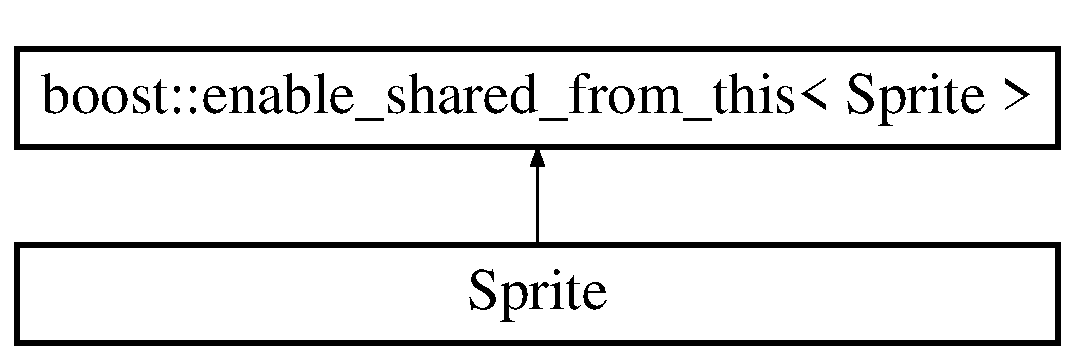
\includegraphics[height=2.000000cm]{class_sprite}
\end{center}
\end{figure}
\subsection*{Public Member Functions}
\begin{DoxyCompactItemize}
\item 
boost\+::shared\+\_\+ptr$<$ \hyperlink{class_sprite}{Sprite} $>$ {\bfseries Get\+Ptr} ()\hypertarget{class_sprite_af2665e7f459c2df1b74e69daaf44c19a}{}\label{class_sprite_af2665e7f459c2df1b74e69daaf44c19a}

\item 
void {\bfseries Set\+Pos} (float x, float y)\hypertarget{class_sprite_afea5e8f8f745b1db09b86f45943283af}{}\label{class_sprite_afea5e8f8f745b1db09b86f45943283af}

\item 
void {\bfseries Set\+Pos} (float x, float y, float z)\hypertarget{class_sprite_a31d06db54797d787445bee85b71f5dcd}{}\label{class_sprite_a31d06db54797d787445bee85b71f5dcd}

\item 
std\+::string const {\bfseries Get\+Name} ()\hypertarget{class_sprite_aa590f40b37b1a933aa373d907f5c8ae5}{}\label{class_sprite_aa590f40b37b1a933aa373d907f5c8ae5}

\item 
void {\bfseries Set\+Name} (std\+::string name)\hypertarget{class_sprite_a03e3fa1da28c44d7731cf09bba12fa08}{}\label{class_sprite_a03e3fa1da28c44d7731cf09bba12fa08}

\item 
float const {\bfseries GetX} ()\hypertarget{class_sprite_ad878be7d0af1494307f89cc8b4d06dbf}{}\label{class_sprite_ad878be7d0af1494307f89cc8b4d06dbf}

\item 
void {\bfseries SetX} (float x)\hypertarget{class_sprite_a87a083a64e6684aa8c5fe9965f3093af}{}\label{class_sprite_a87a083a64e6684aa8c5fe9965f3093af}

\item 
float const {\bfseries GetY} ()\hypertarget{class_sprite_ab639bc265bb54792c4bbf64dca743139}{}\label{class_sprite_ab639bc265bb54792c4bbf64dca743139}

\item 
void {\bfseries SetY} (float y)\hypertarget{class_sprite_ab5d4b3fd91f5c6d5bed02bf5eaf386ab}{}\label{class_sprite_ab5d4b3fd91f5c6d5bed02bf5eaf386ab}

\item 
float const {\bfseries GetZ} ()\hypertarget{class_sprite_a2aeadc82324dd417bd34e0e915dafecb}{}\label{class_sprite_a2aeadc82324dd417bd34e0e915dafecb}

\item 
void {\bfseries SetZ} (float z)\hypertarget{class_sprite_a567604b2b89b44baa6f01bb84da96768}{}\label{class_sprite_a567604b2b89b44baa6f01bb84da96768}

\item 
float const {\bfseries Get\+Alpha} ()\hypertarget{class_sprite_abfa0b7e0e9481a6692f9923db2aa91f0}{}\label{class_sprite_abfa0b7e0e9481a6692f9923db2aa91f0}

\item 
void {\bfseries Set\+Alpha} (float alpha)\hypertarget{class_sprite_a9c313cc32eac1f56890fc4fd8786e13a}{}\label{class_sprite_a9c313cc32eac1f56890fc4fd8786e13a}

\item 
ColorF const {\bfseries Get\+Color} ()\hypertarget{class_sprite_a018bea36d97ae24020766bd4e6bc7916}{}\label{class_sprite_a018bea36d97ae24020766bd4e6bc7916}

\item 
void {\bfseries Set\+Color} (ColorF color)\hypertarget{class_sprite_a840d056169580917d428cab4fe16b57e}{}\label{class_sprite_a840d056169580917d428cab4fe16b57e}

\item 
float const {\bfseries Get\+Width} ()\hypertarget{class_sprite_ac48454d9f731d63bbb587a9b755de579}{}\label{class_sprite_ac48454d9f731d63bbb587a9b755de579}

\item 
void {\bfseries Set\+Width} (float width)\hypertarget{class_sprite_afb09c8cac9d843a2fc55aaad1df77b25}{}\label{class_sprite_afb09c8cac9d843a2fc55aaad1df77b25}

\item 
float const {\bfseries Get\+Height} ()\hypertarget{class_sprite_a52d8add95194880591d25993028d37f7}{}\label{class_sprite_a52d8add95194880591d25993028d37f7}

\item 
void {\bfseries Set\+Height} (float height)\hypertarget{class_sprite_a82d4aa5c5b44955daf604d4668b94882}{}\label{class_sprite_a82d4aa5c5b44955daf604d4668b94882}

\item 
Point2\+DI {\bfseries Get\+Origin\+Tex\+Size} ()\hypertarget{class_sprite_ab5e6db0adf89e3cf653f3f82d86c1246}{}\label{class_sprite_ab5e6db0adf89e3cf653f3f82d86c1246}

\item 
float const {\bfseries Get\+Draw\+Width} ()\hypertarget{class_sprite_afa906d1a181384865893c2b0449c8317}{}\label{class_sprite_afa906d1a181384865893c2b0449c8317}

\item 
void {\bfseries Set\+Draw\+Width} (float width)\hypertarget{class_sprite_abe5a865940faefa441c5a75c221c9298}{}\label{class_sprite_abe5a865940faefa441c5a75c221c9298}

\item 
float const {\bfseries Get\+Draw\+Height} ()\hypertarget{class_sprite_aa715da119494b5adb1b2d45349f43b0e}{}\label{class_sprite_aa715da119494b5adb1b2d45349f43b0e}

\item 
void {\bfseries Set\+Draw\+Height} (float height)\hypertarget{class_sprite_ae7962b547e176617f7fd2c9e7e425426}{}\label{class_sprite_ae7962b547e176617f7fd2c9e7e425426}

\item 
void {\bfseries Set\+Center} (float x, float y)\hypertarget{class_sprite_a7ac80cebb5d5f28ab2368dab973c1024}{}\label{class_sprite_a7ac80cebb5d5f28ab2368dab973c1024}

\item 
float const {\bfseries Get\+CenterX} ()\hypertarget{class_sprite_af706187c7fafdce2735eda41704dd313}{}\label{class_sprite_af706187c7fafdce2735eda41704dd313}

\item 
void {\bfseries Set\+CenterX} (float x)\hypertarget{class_sprite_a77d64ed38fcfe7be5133cd4718ad555a}{}\label{class_sprite_a77d64ed38fcfe7be5133cd4718ad555a}

\item 
float const {\bfseries Get\+CenterY} ()\hypertarget{class_sprite_a02209dd06e503979d253f40adf64e0d3}{}\label{class_sprite_a02209dd06e503979d253f40adf64e0d3}

\item 
void {\bfseries Set\+CenterY} (float y)\hypertarget{class_sprite_afafaa5878dfa4cf152fed8ae250ed3a1}{}\label{class_sprite_afafaa5878dfa4cf152fed8ae250ed3a1}

\item 
float const {\bfseries Get\+Rot} ()\hypertarget{class_sprite_a2396892e7d1e6f23aa0cd4e2f8c98a1e}{}\label{class_sprite_a2396892e7d1e6f23aa0cd4e2f8c98a1e}

\item 
void {\bfseries Set\+Rot} (float rot)\hypertarget{class_sprite_a6ba917cb5b9ee64513b442ffca992c45}{}\label{class_sprite_a6ba917cb5b9ee64513b442ffca992c45}

\item 
float const {\bfseries Get\+Rot\+OffcetX} ()\hypertarget{class_sprite_ae8334552f5e09e1e753d7b7a85dab305}{}\label{class_sprite_ae8334552f5e09e1e753d7b7a85dab305}

\item 
void {\bfseries Set\+Rot\+OffcetX} (float x)\hypertarget{class_sprite_a132e465221d9172fe96407c4ae00d3e3}{}\label{class_sprite_a132e465221d9172fe96407c4ae00d3e3}

\item 
float const {\bfseries Get\+Rot\+OffcetY} ()\hypertarget{class_sprite_a2e2406168106be0c582264f51616cb03}{}\label{class_sprite_a2e2406168106be0c582264f51616cb03}

\item 
void {\bfseries Set\+Rot\+OffcetY} (float y)\hypertarget{class_sprite_a0b8dd8b526142d02f5a49067d3b4c5cf}{}\label{class_sprite_a0b8dd8b526142d02f5a49067d3b4c5cf}

\item 
int const {\bfseries Get\+Div\+Draw\+Tex\+Idx} ()\hypertarget{class_sprite_a05987625c32ec55e2cc980d467396115}{}\label{class_sprite_a05987625c32ec55e2cc980d467396115}

\item 
void {\bfseries Set\+Div\+Draw\+Tex\+Idx} (int idx)\hypertarget{class_sprite_a7921c100391fa7461eedde66287006b5}{}\label{class_sprite_a7921c100391fa7461eedde66287006b5}

\item 
bool \hyperlink{class_sprite_a190e9dc44c2d90ad8f5697995d5be120}{Is\+Draw} () const \hypertarget{class_sprite_a190e9dc44c2d90ad8f5697995d5be120}{}\label{class_sprite_a190e9dc44c2d90ad8f5697995d5be120}

\begin{DoxyCompactList}\small\item\em 表示・非表示の状態を取得する \end{DoxyCompactList}\item 
void \hyperlink{class_sprite_a5b1ddf57e50d7ff6628686c6b5d86efe}{Show} ()\hypertarget{class_sprite_a5b1ddf57e50d7ff6628686c6b5d86efe}{}\label{class_sprite_a5b1ddf57e50d7ff6628686c6b5d86efe}

\begin{DoxyCompactList}\small\item\em 描画する状態にする \end{DoxyCompactList}\item 
void \hyperlink{class_sprite_a0daa142d5c6a7bd99680ab623ad0d61b}{Hide} ()\hypertarget{class_sprite_a0daa142d5c6a7bd99680ab623ad0d61b}{}\label{class_sprite_a0daa142d5c6a7bd99680ab623ad0d61b}

\begin{DoxyCompactList}\small\item\em 描画しない状態にする \end{DoxyCompactList}\item 
void \hyperlink{class_sprite_a0ae1cdfd5e34c1f61ebfe9fd39b0fc72}{Set\+Draw\+Pos\+Absolute} ()\hypertarget{class_sprite_a0ae1cdfd5e34c1f61ebfe9fd39b0fc72}{}\label{class_sprite_a0ae1cdfd5e34c1f61ebfe9fd39b0fc72}

\begin{DoxyCompactList}\small\item\em ウィンドウからの絶対座標で描画する状態にする \end{DoxyCompactList}\item 
void \hyperlink{class_sprite_aec55bcf3fcbe90a59e08c0adf3a7dd62}{Set\+Draw\+Pos\+Relative} ()\hypertarget{class_sprite_aec55bcf3fcbe90a59e08c0adf3a7dd62}{}\label{class_sprite_aec55bcf3fcbe90a59e08c0adf3a7dd62}

\begin{DoxyCompactList}\small\item\em 親スプライトからの相対座標で描画する状態にする \end{DoxyCompactList}\item 
void \hyperlink{class_sprite_a6dcfbb2e57eba1548dc5c244b993fe8a}{Set\+Texture\+Mode} (const char $\ast$name)\hypertarget{class_sprite_a6dcfbb2e57eba1548dc5c244b993fe8a}{}\label{class_sprite_a6dcfbb2e57eba1548dc5c244b993fe8a}

\begin{DoxyCompactList}\small\item\em 指定したエイリアスのテクスチャを用いて、描画モードをテクスチャに設定する \end{DoxyCompactList}\item 
void \hyperlink{class_sprite_a32c37cab456e545730d64c5b87757039}{Set\+Div\+Texture\+Mode} (const char $\ast$name, int xnum, int ynum, int width, int height)
\item 
void \hyperlink{class_sprite_a6a61fed0b01e45a727c79e2847b987c0}{Set\+Texture\+Src} (int x, int y, int w, int h)\hypertarget{class_sprite_a6a61fed0b01e45a727c79e2847b987c0}{}\label{class_sprite_a6a61fed0b01e45a727c79e2847b987c0}

\begin{DoxyCompactList}\small\item\em テクスチャを描画する際、描画に使用する範囲を指定する \end{DoxyCompactList}\item 
void \hyperlink{class_sprite_aa379c17355f7e4c2db4f4b83b12dadf7}{Set\+Texture\+ColorF} (ColorF color)\hypertarget{class_sprite_aa379c17355f7e4c2db4f4b83b12dadf7}{}\label{class_sprite_aa379c17355f7e4c2db4f4b83b12dadf7}

\begin{DoxyCompactList}\small\item\em テクスチャの描画色を設定する \end{DoxyCompactList}\item 
void \hyperlink{class_sprite_ac21f74c27e5470ab2bd54fdfe4de0e3a}{Set\+Text\+Mode} (const char $\ast$text)\hypertarget{class_sprite_ac21f74c27e5470ab2bd54fdfe4de0e3a}{}\label{class_sprite_ac21f74c27e5470ab2bd54fdfe4de0e3a}

\begin{DoxyCompactList}\small\item\em テキスト描画モードにする \end{DoxyCompactList}\item 
void \hyperlink{class_sprite_a8e3565ccc4488800e51b32cdd11a2420}{Set\+Text\+Mode2} (const char $\ast$text, const char $\ast$font)\hypertarget{class_sprite_a8e3565ccc4488800e51b32cdd11a2420}{}\label{class_sprite_a8e3565ccc4488800e51b32cdd11a2420}

\begin{DoxyCompactList}\small\item\em フォントを指定してテキスト描画モードにする \end{DoxyCompactList}\item 
void \hyperlink{class_sprite_a99210c1ece23e87b442d88beabab511d}{Set\+Text} (const char $\ast$text)\hypertarget{class_sprite_a99210c1ece23e87b442d88beabab511d}{}\label{class_sprite_a99210c1ece23e87b442d88beabab511d}

\begin{DoxyCompactList}\small\item\em 描画するテキストを設定する \end{DoxyCompactList}\item 
std\+::string \hyperlink{class_sprite_ada760c966df1e9bf4ae99258ce9d415f}{Get\+Text} ()\hypertarget{class_sprite_ada760c966df1e9bf4ae99258ce9d415f}{}\label{class_sprite_ada760c966df1e9bf4ae99258ce9d415f}

\begin{DoxyCompactList}\small\item\em テキストを取得する \end{DoxyCompactList}\item 
void \hyperlink{class_sprite_aee4258d6eeeff4d498e8b9c2f10be7e2}{Set\+Text\+ColorF} (ColorF color)\hypertarget{class_sprite_aee4258d6eeeff4d498e8b9c2f10be7e2}{}\label{class_sprite_aee4258d6eeeff4d498e8b9c2f10be7e2}

\begin{DoxyCompactList}\small\item\em テキストの描画色を設定する \end{DoxyCompactList}\item 
void \hyperlink{class_sprite_aa888b89fabd743e903efa2402d002f46}{Set\+Text\+Color1} (float r, float g, float b)\hypertarget{class_sprite_aa888b89fabd743e903efa2402d002f46}{}\label{class_sprite_aa888b89fabd743e903efa2402d002f46}

\begin{DoxyCompactList}\small\item\em テキストの描画色を設定する(0.\+0-\/1.\+0) \end{DoxyCompactList}\item 
void \hyperlink{class_sprite_a32887a481da8a5e23e072b3747a8f798}{Set\+Text\+Color255} (int r, int g, int b)\hypertarget{class_sprite_a32887a481da8a5e23e072b3747a8f798}{}\label{class_sprite_a32887a481da8a5e23e072b3747a8f798}

\begin{DoxyCompactList}\small\item\em テキストの描画色を設定する(0-\/255) \end{DoxyCompactList}\item 
void \hyperlink{class_sprite_a13145ca2b7ad2f0881f2a06b31fa2937}{Set\+Font\+Size} (int size)\hypertarget{class_sprite_a13145ca2b7ad2f0881f2a06b31fa2937}{}\label{class_sprite_a13145ca2b7ad2f0881f2a06b31fa2937}

\begin{DoxyCompactList}\small\item\em テキスト描画のフォントサイズを設定する \end{DoxyCompactList}\item 
void \hyperlink{class_sprite_ad90bd4a0eda1d12d37c4e740ce4c69d5}{Add\+Child} (boost\+::shared\+\_\+ptr$<$ \hyperlink{class_sprite}{Sprite} $>$ chr)\hypertarget{class_sprite_ad90bd4a0eda1d12d37c4e740ce4c69d5}{}\label{class_sprite_ad90bd4a0eda1d12d37c4e740ce4c69d5}

\begin{DoxyCompactList}\small\item\em 子スプライトを追加する \end{DoxyCompactList}\item 
void \hyperlink{class_sprite_a25d21de7dc41150e49d10374c6fe227b}{Remove\+Child} (boost\+::shared\+\_\+ptr$<$ \hyperlink{class_sprite}{Sprite} $>$ chr)\hypertarget{class_sprite_a25d21de7dc41150e49d10374c6fe227b}{}\label{class_sprite_a25d21de7dc41150e49d10374c6fe227b}

\begin{DoxyCompactList}\small\item\em 子スプライトを削除する \end{DoxyCompactList}\item 
void \hyperlink{class_sprite_a063c4d0a341d1ea48e17f3baa4f420a0}{Clear\+Child} ()\hypertarget{class_sprite_a063c4d0a341d1ea48e17f3baa4f420a0}{}\label{class_sprite_a063c4d0a341d1ea48e17f3baa4f420a0}

\begin{DoxyCompactList}\small\item\em 子スプライトを全て削除する \end{DoxyCompactList}\item 
void \hyperlink{class_sprite_a35deac40351bf9902cf89985ace6cdce}{Set\+Parent} (boost\+::shared\+\_\+ptr$<$ \hyperlink{class_sprite}{Sprite} $>$ parent)\hypertarget{class_sprite_a35deac40351bf9902cf89985ace6cdce}{}\label{class_sprite_a35deac40351bf9902cf89985ace6cdce}

\begin{DoxyCompactList}\small\item\em 親スプライトを設定する \end{DoxyCompactList}\item 
void \hyperlink{class_sprite_a5cff0acb60cc920ba029370cf51189d6}{Remove\+From\+Parent} ()\hypertarget{class_sprite_a5cff0acb60cc920ba029370cf51189d6}{}\label{class_sprite_a5cff0acb60cc920ba029370cf51189d6}

\begin{DoxyCompactList}\small\item\em 親スプライトから自身を切り離す \end{DoxyCompactList}\item 
void \hyperlink{class_sprite_a4ac35f129e53066caed4095346436988}{Remove\+From\+Parent\+Force} ()\hypertarget{class_sprite_a4ac35f129e53066caed4095346436988}{}\label{class_sprite_a4ac35f129e53066caed4095346436988}

\begin{DoxyCompactList}\small\item\em 親スプライトから自身を強制的に切り離す(基本的に呼び出さないこと) \end{DoxyCompactList}\item 
int \hyperlink{class_sprite_ab3c4588051c85b918427f2fc7418bc02}{Get\+Child\+Cnt} ()\hypertarget{class_sprite_ab3c4588051c85b918427f2fc7418bc02}{}\label{class_sprite_ab3c4588051c85b918427f2fc7418bc02}

\begin{DoxyCompactList}\small\item\em 子スプライトの数を取得する \end{DoxyCompactList}\item 
boost\+::shared\+\_\+ptr$<$ \hyperlink{class_sprite}{Sprite} $>$ \hyperlink{class_sprite_a6a749d3a10f96778d41c215fbc44febc}{Get\+Child} (int idx)\hypertarget{class_sprite_a6a749d3a10f96778d41c215fbc44febc}{}\label{class_sprite_a6a749d3a10f96778d41c215fbc44febc}

\begin{DoxyCompactList}\small\item\em 子スプライトを取得する \end{DoxyCompactList}\item 
void \hyperlink{class_sprite_a876a63cc6e81caf295fbeb45563b2de6}{Draw\+This} (Engine\+::\+Graphics\+::\+Simple\+::\+I\+Sprite\+Renderer $\ast$p\+Spr, float baseX, float baseY)\hypertarget{class_sprite_a876a63cc6e81caf295fbeb45563b2de6}{}\label{class_sprite_a876a63cc6e81caf295fbeb45563b2de6}

\begin{DoxyCompactList}\small\item\em 自身を描画する \end{DoxyCompactList}\item 
void \hyperlink{class_sprite_ad397965cd4e7cfc0c1fc9fead78c757d}{Draw} (Engine\+::\+Graphics\+::\+Simple\+::\+I\+Sprite\+Renderer $\ast$p\+Spr, float baseX, float baseY, int level)\hypertarget{class_sprite_ad397965cd4e7cfc0c1fc9fead78c757d}{}\label{class_sprite_ad397965cd4e7cfc0c1fc9fead78c757d}

\begin{DoxyCompactList}\small\item\em 子スプライトを含めて描画する \end{DoxyCompactList}\item 
void \hyperlink{class_sprite_a24a595468adde636a8b820874e20e1ca}{SortZ} ()\hypertarget{class_sprite_a24a595468adde636a8b820874e20e1ca}{}\label{class_sprite_a24a595468adde636a8b820874e20e1ca}

\begin{DoxyCompactList}\small\item\em 子スプライトを\+Z座標でソートする(Z座標が小さいほど手前に描画される) \end{DoxyCompactList}\item 
RectI \hyperlink{class_sprite_a5c2932082f60140474753006a3897287}{Get\+Bounds} ()\hypertarget{class_sprite_a5c2932082f60140474753006a3897287}{}\label{class_sprite_a5c2932082f60140474753006a3897287}

\begin{DoxyCompactList}\small\item\em 描画領域の大きさを取得する \end{DoxyCompactList}\end{DoxyCompactItemize}
\subsection*{Static Public Member Functions}
\begin{DoxyCompactItemize}
\item 
static void \hyperlink{class_sprite_a15b80053ef337d4f35eed273302773ff}{Regist\+Lua} ()\hypertarget{class_sprite_a15b80053ef337d4f35eed273302773ff}{}\label{class_sprite_a15b80053ef337d4f35eed273302773ff}

\begin{DoxyCompactList}\small\item\em Luaで使用する機能を登録する \end{DoxyCompactList}\end{DoxyCompactItemize}
\subsection*{Protected Types}
\begin{DoxyCompactItemize}
\item 
enum \hyperlink{class_sprite_a7e6c7652514341b0ccd721166a1d00d1}{Mode} \{ {\bfseries S\+P\+R\+\_\+\+N\+O\+NE}, 
\hyperlink{class_sprite_a7e6c7652514341b0ccd721166a1d00d1a8396f95eb7d47c37ce60278c02644cb3}{S\+P\+R\+\_\+\+T\+E\+X\+T\+U\+RE}, 
\hyperlink{class_sprite_a7e6c7652514341b0ccd721166a1d00d1ab595e70dfd597d3d95865920928895cb}{S\+P\+R\+\_\+\+T\+E\+XT}
 \}\begin{DoxyCompactList}\small\item\em 表示モードを示す \end{DoxyCompactList}
\item 
typedef std\+::list$<$ boost\+::shared\+\_\+ptr$<$ \hyperlink{class_sprite}{Sprite} $>$ $>$\+::iterator {\bfseries Itr}\hypertarget{class_sprite_ac12e68e5dd906ef304b5e4997400371d}{}\label{class_sprite_ac12e68e5dd906ef304b5e4997400371d}

\end{DoxyCompactItemize}
\subsection*{Protected Member Functions}
\begin{DoxyCompactItemize}
\item 
void \hyperlink{class_sprite_a8b785863b8ac6c285512a0c842d0fdbb}{Update\+Size} ()\hypertarget{class_sprite_a8b785863b8ac6c285512a0c842d0fdbb}{}\label{class_sprite_a8b785863b8ac6c285512a0c842d0fdbb}

\begin{DoxyCompactList}\small\item\em 設定されたテクスチャ情報を用いて、自身が保持する大きさの情報を更新する。 \end{DoxyCompactList}\end{DoxyCompactItemize}
\subsection*{Protected Attributes}
\begin{DoxyCompactItemize}
\item 
\hyperlink{class_sprite_a7e6c7652514341b0ccd721166a1d00d1}{Mode} {\bfseries m\+\_\+mode}\hypertarget{class_sprite_ada9da6a8ed8b81539e86b8ab0dde9d69}{}\label{class_sprite_ada9da6a8ed8b81539e86b8ab0dde9d69}

\item 
bool {\bfseries m\+\_\+is\+Draw}\hypertarget{class_sprite_ac9390a7e9c4605d29d888dcad59af234}{}\label{class_sprite_ac9390a7e9c4605d29d888dcad59af234}

\item 
Draw\+Pos\+Type {\bfseries m\+\_\+pos\+Type}\hypertarget{class_sprite_a23c37ce224637ae1f3fa146925618fc3}{}\label{class_sprite_a23c37ce224637ae1f3fa146925618fc3}

\item 
std\+::string {\bfseries m\+\_\+name}\hypertarget{class_sprite_aa62f8c64b12839b25ac67e2afbf2f040}{}\label{class_sprite_aa62f8c64b12839b25ac67e2afbf2f040}

\item 
float {\bfseries m\+\_\+alpha}\hypertarget{class_sprite_af13153e7ee278203552cf477cabda410}{}\label{class_sprite_af13153e7ee278203552cf477cabda410}

\item 
float {\bfseries m\+\_\+x}\hypertarget{class_sprite_a41e98ab9be3404db1fc7037bee042ab1}{}\label{class_sprite_a41e98ab9be3404db1fc7037bee042ab1}

\item 
float {\bfseries m\+\_\+y}\hypertarget{class_sprite_a62184d5c7605e5bd49b284c6249cb965}{}\label{class_sprite_a62184d5c7605e5bd49b284c6249cb965}

\item 
float {\bfseries m\+\_\+z}\hypertarget{class_sprite_a9cca3a51a0392d947676cc3c9858c778}{}\label{class_sprite_a9cca3a51a0392d947676cc3c9858c778}

\item 
float {\bfseries m\+\_\+width}\hypertarget{class_sprite_aff10eb00cfd126b2433c72148d71c8d0}{}\label{class_sprite_aff10eb00cfd126b2433c72148d71c8d0}

\item 
float {\bfseries m\+\_\+height}\hypertarget{class_sprite_a43feb4c9a3898a47c9a739b5912ddad7}{}\label{class_sprite_a43feb4c9a3898a47c9a739b5912ddad7}

\item 
float {\bfseries m\+\_\+draw\+Width}\hypertarget{class_sprite_add09b3c31ba419b81d8ae0acdfee33c9}{}\label{class_sprite_add09b3c31ba419b81d8ae0acdfee33c9}

\item 
float {\bfseries m\+\_\+draw\+Height}\hypertarget{class_sprite_a0b4b47e53f0b5bfeb5d6260298b36dea}{}\label{class_sprite_a0b4b47e53f0b5bfeb5d6260298b36dea}

\item 
float {\bfseries m\+\_\+centerX}\hypertarget{class_sprite_a7747583d8bcdb8ee521e7866049218e1}{}\label{class_sprite_a7747583d8bcdb8ee521e7866049218e1}

\item 
float {\bfseries m\+\_\+centerY}\hypertarget{class_sprite_abf5bc5a5f4ed5086da3508cef8ee9602}{}\label{class_sprite_abf5bc5a5f4ed5086da3508cef8ee9602}

\item 
float {\bfseries m\+\_\+rot}\hypertarget{class_sprite_a068051f63c91c7c497865b37812565e1}{}\label{class_sprite_a068051f63c91c7c497865b37812565e1}

\item 
float {\bfseries m\+\_\+rot\+OffcetX}\hypertarget{class_sprite_ad11d48338e82f142bceaaa36f45c5669}{}\label{class_sprite_ad11d48338e82f142bceaaa36f45c5669}

\item 
float {\bfseries m\+\_\+rot\+OffcetY}\hypertarget{class_sprite_aee6c233e07c4c154868bb75db0903db7}{}\label{class_sprite_aee6c233e07c4c154868bb75db0903db7}

\item 
int {\bfseries m\+\_\+div\+Draw\+Tex\+Idx}\hypertarget{class_sprite_a890a208987d08676ca568b3d9e832059}{}\label{class_sprite_a890a208987d08676ca568b3d9e832059}

\item 
int {\bfseries m\+\_\+divX}\hypertarget{class_sprite_a5835815afe183734d4b2895509c7717f}{}\label{class_sprite_a5835815afe183734d4b2895509c7717f}

\item 
int {\bfseries m\+\_\+divY}\hypertarget{class_sprite_ae1ced55597bd91f128bd6dc92162430a}{}\label{class_sprite_ae1ced55597bd91f128bd6dc92162430a}

\item 
int {\bfseries m\+\_\+divW}\hypertarget{class_sprite_ae56e8dfc134772a5208c1ed43c1e7a59}{}\label{class_sprite_ae56e8dfc134772a5208c1ed43c1e7a59}

\item 
int {\bfseries m\+\_\+divH}\hypertarget{class_sprite_a32a9fe14ba4a968560c8bf16a514c632}{}\label{class_sprite_a32a9fe14ba4a968560c8bf16a514c632}

\item 
int {\bfseries m\+\_\+srcX}\hypertarget{class_sprite_a6d9092d0007588dff19470a7f550a37e}{}\label{class_sprite_a6d9092d0007588dff19470a7f550a37e}

\item 
int {\bfseries m\+\_\+srcY}\hypertarget{class_sprite_a716aa1d64bf6ac00379f081259fde67b}{}\label{class_sprite_a716aa1d64bf6ac00379f081259fde67b}

\item 
int {\bfseries m\+\_\+srcW}\hypertarget{class_sprite_a97bafb109664b59eb7ca390c5cead173}{}\label{class_sprite_a97bafb109664b59eb7ca390c5cead173}

\item 
int {\bfseries m\+\_\+srcH}\hypertarget{class_sprite_a9ac3b201e89ec36289e07d1c2fd5eb2e}{}\label{class_sprite_a9ac3b201e89ec36289e07d1c2fd5eb2e}

\item 
Engine\+::\+Graphics\+::\+Resource\+::\+I\+Texture $\ast$ {\bfseries m\+\_\+p\+Tex\+Buf}\hypertarget{class_sprite_a6dcba95237c988ed4d993a8ff4ca658f}{}\label{class_sprite_a6dcba95237c988ed4d993a8ff4ca658f}

\item 
ColorF {\bfseries m\+\_\+texture\+Color}\hypertarget{class_sprite_aea3e77cd97e5cc826a07475ac06f3f7c}{}\label{class_sprite_aea3e77cd97e5cc826a07475ac06f3f7c}

\item 
Texture\+Div\+Type {\bfseries m\+\_\+div\+Type}\hypertarget{class_sprite_a9fd5ed190dec101502564732eaba8427}{}\label{class_sprite_a9fd5ed190dec101502564732eaba8427}

\item 
bool {\bfseries m\+\_\+use\+Text\+Renderer}\hypertarget{class_sprite_afc5e6315b779d8550fd081079984b209}{}\label{class_sprite_afc5e6315b779d8550fd081079984b209}

\item 
Engine\+::\+Graphics\+::\+Simple\+::\+I\+Text\+Renderer $\ast$ {\bfseries m\+\_\+p\+Text\+Rdr}\hypertarget{class_sprite_a4d3975b753781c3eb457539bea6c80fe}{}\label{class_sprite_a4d3975b753781c3eb457539bea6c80fe}

\item 
Graphics\+::\+Resource\+::\+Text\+::\+I\+Text\+Data $\ast$ {\bfseries m\+\_\+p\+Text\+Data}\hypertarget{class_sprite_aba79582eaee4411ad7971f706a259f70}{}\label{class_sprite_aba79582eaee4411ad7971f706a259f70}

\item 
wchar\+\_\+t {\bfseries m\+\_\+text} \mbox{[}M\+A\+X\+\_\+\+T\+E\+XT\mbox{]}\hypertarget{class_sprite_a7e22779568fcb5455c0c95b72e055b27}{}\label{class_sprite_a7e22779568fcb5455c0c95b72e055b27}

\item 
ColorF {\bfseries m\+\_\+text\+Color}\hypertarget{class_sprite_a5715eb71948a9edbd58d0e4bb6f55f3e}{}\label{class_sprite_a5715eb71948a9edbd58d0e4bb6f55f3e}

\item 
std\+::string {\bfseries m\+\_\+font\+Name}\hypertarget{class_sprite_a332be0e92f2fe2dbb72d1590a42af9eb}{}\label{class_sprite_a332be0e92f2fe2dbb72d1590a42af9eb}

\item 
int {\bfseries m\+\_\+font\+Size}\hypertarget{class_sprite_abe9f44c7754c66469f3bd55e626beaa5}{}\label{class_sprite_abe9f44c7754c66469f3bd55e626beaa5}

\item 
boost\+::weak\+\_\+ptr$<$ \hyperlink{class_sprite}{Sprite} $>$ {\bfseries m\+\_\+p\+Parent}\hypertarget{class_sprite_a8f9fc0b824deb7d61fbbdbf8efc471a5}{}\label{class_sprite_a8f9fc0b824deb7d61fbbdbf8efc471a5}

\item 
std\+::list$<$ boost\+::shared\+\_\+ptr$<$ \hyperlink{class_sprite}{Sprite} $>$ $>$ {\bfseries m\+\_\+children}\hypertarget{class_sprite_a3d1fc94c57d9516cdef1a16f73c87e70}{}\label{class_sprite_a3d1fc94c57d9516cdef1a16f73c87e70}

\end{DoxyCompactItemize}
\subsection*{Static Protected Attributes}
\begin{DoxyCompactItemize}
\item 
static const int {\bfseries M\+A\+X\+\_\+\+T\+E\+XT} = 256\hypertarget{class_sprite_afc635126006821982a8dfece2b8acafc}{}\label{class_sprite_afc635126006821982a8dfece2b8acafc}

\end{DoxyCompactItemize}


\subsection{Detailed Description}
スプライト機能を提供する 

\subsection{Member Enumeration Documentation}
\index{Sprite@{Sprite}!Mode@{Mode}}
\index{Mode@{Mode}!Sprite@{Sprite}}
\subsubsection[{\texorpdfstring{Mode}{Mode}}]{\setlength{\rightskip}{0pt plus 5cm}enum {\bf Sprite\+::\+Mode}\hspace{0.3cm}{\ttfamily [protected]}}\hypertarget{class_sprite_a7e6c7652514341b0ccd721166a1d00d1}{}\label{class_sprite_a7e6c7652514341b0ccd721166a1d00d1}


表示モードを示す 

\begin{Desc}
\item[Enumerator]\par
\begin{description}
\index{S\+P\+R\+\_\+\+T\+E\+X\+T\+U\+RE@{S\+P\+R\+\_\+\+T\+E\+X\+T\+U\+RE}!Sprite@{Sprite}}\index{Sprite@{Sprite}!S\+P\+R\+\_\+\+T\+E\+X\+T\+U\+RE@{S\+P\+R\+\_\+\+T\+E\+X\+T\+U\+RE}}\item[{\em 
S\+P\+R\+\_\+\+T\+E\+X\+T\+U\+RE\hypertarget{class_sprite_a7e6c7652514341b0ccd721166a1d00d1a8396f95eb7d47c37ce60278c02644cb3}{}\label{class_sprite_a7e6c7652514341b0ccd721166a1d00d1a8396f95eb7d47c37ce60278c02644cb3}
}]非表示 \index{S\+P\+R\+\_\+\+T\+E\+XT@{S\+P\+R\+\_\+\+T\+E\+XT}!Sprite@{Sprite}}\index{Sprite@{Sprite}!S\+P\+R\+\_\+\+T\+E\+XT@{S\+P\+R\+\_\+\+T\+E\+XT}}\item[{\em 
S\+P\+R\+\_\+\+T\+E\+XT\hypertarget{class_sprite_a7e6c7652514341b0ccd721166a1d00d1ab595e70dfd597d3d95865920928895cb}{}\label{class_sprite_a7e6c7652514341b0ccd721166a1d00d1ab595e70dfd597d3d95865920928895cb}
}]テクスチャ描画 \end{description}
\end{Desc}


\subsection{Member Function Documentation}
\index{Sprite@{Sprite}!Set\+Div\+Texture\+Mode@{Set\+Div\+Texture\+Mode}}
\index{Set\+Div\+Texture\+Mode@{Set\+Div\+Texture\+Mode}!Sprite@{Sprite}}
\subsubsection[{\texorpdfstring{Set\+Div\+Texture\+Mode(const char $\ast$name, int xnum, int ynum, int width, int height)}{SetDivTextureMode(const char *name, int xnum, int ynum, int width, int height)}}]{\setlength{\rightskip}{0pt plus 5cm}void Sprite\+::\+Set\+Div\+Texture\+Mode (
\begin{DoxyParamCaption}
\item[{const char $\ast$}]{name, }
\item[{int}]{xnum, }
\item[{int}]{ynum, }
\item[{int}]{width, }
\item[{int}]{height}
\end{DoxyParamCaption}
)}\hypertarget{class_sprite_a32c37cab456e545730d64c5b87757039}{}\label{class_sprite_a32c37cab456e545730d64c5b87757039}
等分割したテクスチャを描画するモードの切替える 
\begin{DoxyParams}{Parameters}
{\em name} & テクスチャのエイリアス \\
\hline
{\em xnum} & X方向の分割数 \\
\hline
{\em ynum} & Y方向の分割数 \\
\hline
{\em width} & 分割後のテクスチャの幅(除算による誤差の影響を抑えるために必要) \\
\hline
{\em height} & 分割後のテクスチャの高さ(除算による誤差の影響を抑えるために必要) \\
\hline
\end{DoxyParams}


The documentation for this class was generated from the following files\+:\begin{DoxyCompactItemize}
\item 
山火-\/ヤギの咆哮-\//Sprite\+Node.\+hpp\item 
山火-\/ヤギの咆哮-\//Sprite\+Node.\+cpp\end{DoxyCompactItemize}

%--- End generated contents ---

% Index
\backmatter
\newpage
\phantomsection
\clearemptydoublepage
\addcontentsline{toc}{chapter}{Index}
\printindex

\end{document}
